\section{Situando semillas}
Como ya dijimos, la materia gris est\'a compuesta principalmente por neuronas,
y la materia blanca por axones que las comunican. Por ello es com\'un situar
las semillas en la interfaz entre las dos materias.  
En [pedir paper a demian] muestran que la materia blanca cercana a la materia gris 
est\'a interconectada por peque\~nos axones. Como estamos interesados en realizar
un estudio de las conexiones entre regiones distantes del cerebro, decidimos
situar las semillas a \textit{3mm} de la corteza, evitando as\'i el efecto de
\'estos axones locales. El problema es que la corteza del cerebro no es uniforme,
sino que est\'a llena de surcos y ondulaciones. Calcular la distancia entonces
no es inmediato, necesita un m\'etodo que tome estas propiedades en cuenta. 

El primer intento consisti\'o en tomar la parcelaci\'on del sujeto; quedarnos solo 
con la materia blanca y calcular el borde de la misma; generar un
mapa de distancias sobre la materia blanca y quedarnos con los voxels que est\'an
a la distancia deseada. 

Obtuvimos el borde de la materia blanca mediante erosi\'on binaria. La erosi\'on
es una de las dos operaciones morfol\'ogicas b\'asicas en el procesamiento de
im\'agenes \cite{Serra1983}. Dada una imagen binaria $A$ y una estructura binaria
$B$ se define la erosi\'on $ A \ominus B $ como el proceso iterativo de centrar
la estructura $B$ en cada voxel $v$ que vale uno de $A$, si existe un elemento
superpuesto entre $A$ y $B$ donde $B$ vale uno y $A$ vale cero, entonces cambiar
$v$ a cero. \\

\begin{figure}[h!]
                                                                                                                        
\begin{minipage}[b]{\textwidth}
    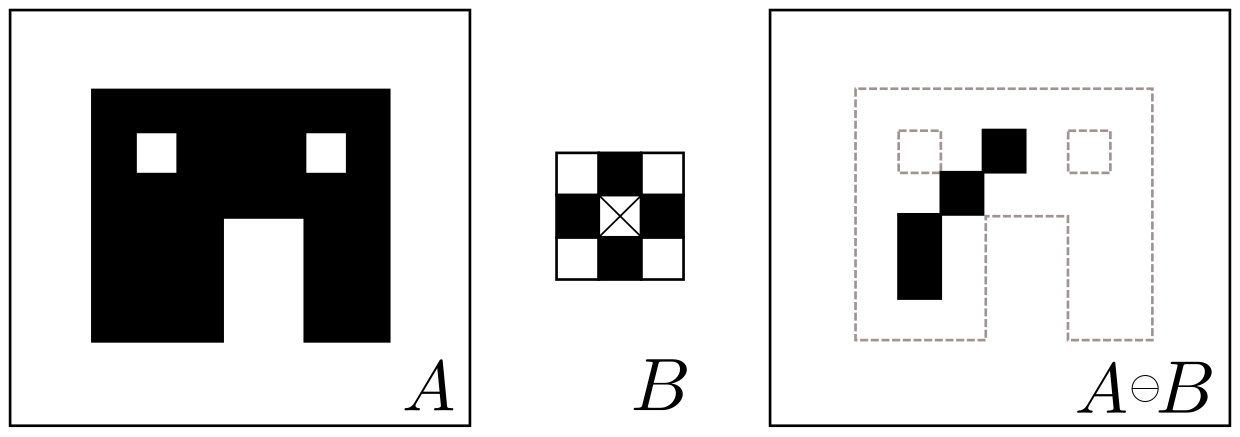
\includegraphics[width=\textwidth]{img/erosion.png}
    \caption{Ejemplo de erosi\'on en imagen binaria}
\end{minipage} ~

\end{figure}  

El mapa de distancias fue generado utilizando el \textit{Fast Marching Method}. 
\textit{FMM} es un m\'etodo para resolver num\'ericamente una versi\'on 
restringida de la ecuaci\'on \textit{Eikonal}. La misma, en su forma general, es
una ecuaci\'on diferencial no lineal que se encuentra com\'unmente en problemas de
propagaci\'on de onda. Tiene la forma: 

$$ V(x) | \nabla u(x) | = F(x) , x \in \Omega $$ 

Donde $\Omega$ es un subconjunto abierto de $R^n$ con un
\textit{buen comportamiento} en su borde. $F(x)$ se denomina el costo temporal y
$V(x)$ es la velocidad de la onda en cada punto. En el caso particular que
queremos resolver $u(x_\omega) = 0, x \in \delta\Omega$;  $F(x)=1$ y $V(x)=1$,
por lo que la ecuaci\'on se resume a:

$$ | \nabla u(x) | = 1 , x \in \Omega $$ 

$u(v)$ en este caso representa el tiempo que tarda la onda en llegar desde
alg\'un elemento del borde hasta el punto $v$ movi\'endose a velocidad constante
de una unidad de espacio por unidad de tiempo. Dada la forma de la velocidad, 
$u(v)$ tambi\'en representa la distancia mas corta que existe entre cualquier
punto $v$ de la imagen y el borde de $\Omega$. \textit{FMM} resuelve este problema
en tiempo $O(n log(n))$ \cite{Sethian2001}, siendo $n$ la cantidad de voxels de 
la imagen.

\begin{figure}[h!]
                                                                                                                        
\begin{minipage}[b]{\textwidth}
    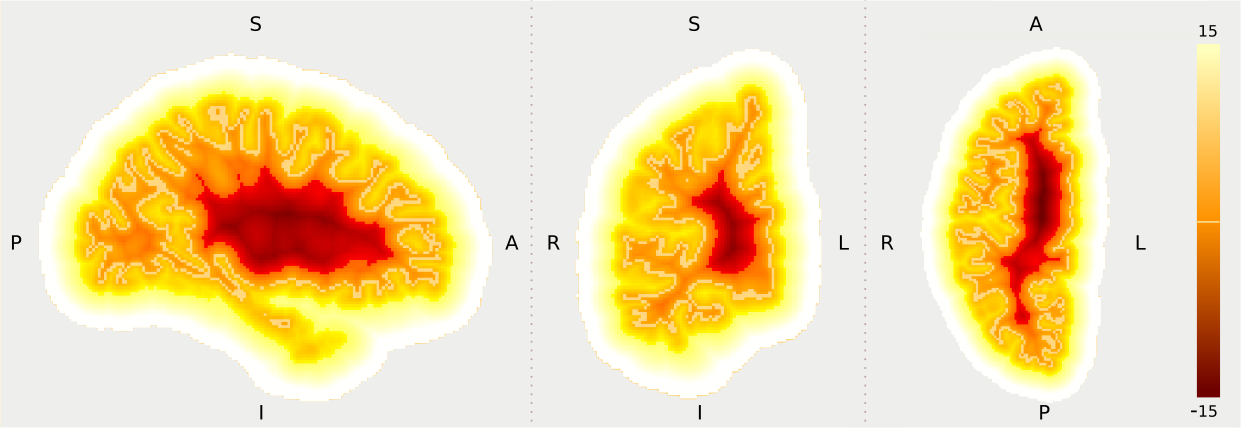
\includegraphics[width=\textwidth]{img/fmm.png}
    \caption{FMM sobre el hemisferio derecho, el borde la materia blanca fue
    resaltado intensionalmente}
\end{minipage} ~

\end{figure}  


El problema de esta primer m\'etodo es que el borde de la materia blanca calculado
de esta manera no coincide con el borde de la corteza definido en la superficie
\textit{Gifti}, lo cual trae problemas al momento de querer mapear las parcelas
obtenidos una vez finalizado todo el proceso de \textit{clustering}. Por este
motivo la segunda soluci\'on propuesta fue: tomar los puntos definidos en la 
superficie, transformarlos al espacio MNI y luego transformarlos nuevamente al 
espacio donde est\'an las im\'agenes de HCP. Usando estos como borde, calcular 
el mapa de distancias sobre la materia blanca utilizando nuevamente \textit{FMM}
y el campo gradiente del mapa. Por la forma que posee el mapa, comenzar desde un
punto del borde y caminar siguiendo el gradiente nos permite adentrarnos en la 
materia blanca respetando la morfolog\'ia de la misma. El proceder de esta manera
nos permite guardar un mapeo entre los valores en la superficie y la posici\'on
de las semillas.\\

Una forma r\'apida y sencilla de validar el correcto funcionamiento del algoritmo
es, partiendo de la parcelaci\'on que ya existe, pintar cada semilla resultante 
del color de la parcela de la cual se comenz\'o. Las semillas generadas
deber\'ian estar a la distancia deseada de la corteza, compartiendo el color de
alguna de las parcelas mas cercanas.
